%! TEX program = lualatex
%        File: main.tex
%     Created: Mar Apr 18 06:00 pm 2017 C
% Last Change: Mar Apr 18 06:00 pm 2017 C
%
\documentclass[11pt, a4paper]{book}
	%\usepackage{pdfsync}
	%\synctex1
	%\usepackage[binding=5mm]{layaureo}
	%\usepackage[marginparwidth=2cm]{geometry}
	\usepackage{marginnote}
	\renewcommand*{\marginfont}{\scshape}
	\pagestyle{plain}
	%\usepackage{syntonly}
	%\syntaxonly
	\usepackage[hidelinks]{hyperref}
	\usepackage{graphicx}
	\usepackage{subfigure}
	\usepackage{xcolor}
	\usepackage{amsmath, amssymb}
		\renewcommand{\epsilon}{\varepsilon}
		\renewcommand{\theta}{\vartheta}
		\renewcommand{\rho}{\varrho}
		\renewcommand{\phi}{\varphi}
	%%%%%%%%%%%%%%%%%%%%%%%%%%%%%%%%%%%%%%%%%
	\usepackage[UKenglish]{babel}
	\usepackage[utf8]{inputenc}
	\usepackage[T1]{fontenc}
	%\usepackage{lmodern}
	\usepackage[lining]{libertine}
	\usepackage[cmbraces, libertine, varg, smallerops]{newtxmath}
	\usepackage{bm}
	\renewcommand{\mathbf}{\bm}
	\usepackage{ebgaramond}
	\usepackage{microtype}
%	\usepackage{titlesec}
%		\titleformat*{\section}{\Large\swshape}
%		\titleformat*{\subsection}{\large\scshape}
%		\titleformat*{\subsubsection}{\scshape}
	\usepackage{fontspec}
	\setmonofont[Scale=MatchLowercase]{Inconsolata}
	%%%%%%%%%%%%%%%%%%%%%%%%%%%%%%%%%%%%%%%%%
	\usepackage{indentfirst}
	%\usepackage[parfill]{parskip}
	\usepackage{booktabs}
	\usepackage[labelfont=bf]{caption}
	\usepackage{multirow}
	\captionsetup[table]{position=top}
	\usepackage{tikz}
	\usepackage{pgfplots}
	\usepackage[mode=image]{standalone}
	%\usepackage{adjustbox}
	\newcommand{\gerda}{\textsc{Gerda}}
	\newcommand{\nbb}{\nu\beta\beta}
	\newcommand{\aof}{\mathring{a}_\text{of}^{(3)}}
	\usepackage[version=4]{mhchem}
	%\usepackage{listings}
	%\lstset{language=C++}
	%\lstset{
	%        basicstyle=\small\ttfamily,
	%        keywordstyle=\color{blue}\bfseries,
	%        commentstyle=\color{darkgray},
	%        stringstyle=\color{orange}
	%        }
	\usepackage{multicol}
\begin{document}
\begin{titlepage}
	\thispagestyle{empty}
	\begin{center}
	
\includegraphics[width=3.5cm]{img/logo.pdf} \\
	\vspace{1cm}
	\textsl{Universit\`a degli Studi di Padova} \\
	\textsl{Dipartimento di Fisica e Astronomia ``Galileo Galilei''} \\
	\vspace{11pt}
	\textsc{Tesi di Laurea Magistrale} \\
	\vspace{3cm}
	\LARGE{Search for Lorentz and CPT symmetries violation in double-beta decay using data from the \textsc{Gerda} experiment}
	\end{center}
	%\vspace{1cm}
	%\begin{center}\textbf{Abstract}\end{center}
	%\small{In the last years a dedicated experimental program searching for neutrinoless double beta decay has started. A careful study of two-neutrino double beta decay is also performed by these experiments because it constitutes a background for the neutrinoless mode. The high precision of many experiments has motivated the formulation of different modes of double-beta decay so that experiments can also look for new physics through unconventional decay modes. In this work we evaluate the presence of a Lorentz and CPT violating double beta decay mode, governed by the $\aof$ parameter, in data coming from the \textsc{Gerda} experiment through a Bayesian statistical analysis.} \\
	%\small{A central goal in modern physics is the development of a unified theory of quantum mechanics and general relativity, many approaches have been developed to combine these two descriptions of nature. It was discovered that many formulations of quantum gravity foresee the breakdown of Lorentz and CPT (the combination of Charge, Parity and Time-reversal transformations) symmetries at the Planck scale, however, the Standard Model (SM) of particle physics assumes a complete invariance under Lorentz transformations and hence CPT transformations. Direct observations at the Planck scale are not yet possible, instead it is possible that physics beyond the SM at very high energies can produce effects at lower energies, observable in current experiments. Some theoretical models predict such low energy effects to show up in the neutrino sector: for example, such effects could produce some distortions in the energy spectrum of the two neutrino double-beta decay process. In this work we evaluate the presence of a Lorentz and CPT violating double-beta decay mode using data coming from the second Phase of the \textsc{Gerda} experiment at LNGS in Italy.} \\
	\vspace{3cm}
	\begin{multicols}{2}
	\noindent
	\textsl{Candidato} \\
	\textsc{Luigi Pertoldi}
	\columnbreak
	\flushright
	\textsl{Relatore} \\
	\textsc{Riccardo Brugnera} \\
	\vspace{5mm}
	\textsl{Corelatore} \\
	\textsc{Katharina von Sturm}
	\end{multicols}
\end{titlepage}
%\tableofcontents
%\listoftables
%\listoffigures
%%! TEX root = ../main.tex
\section*{Introduction}
\addcontentsline{toc}{section}{Introduction}
	%The Standard Model of particle physics, which describes the particles we now believe to be fundamental and their interactions, represents one of the greatest successes of physics of the last century. From the beginning of the debate towards the particle or wave nature of light to the very recent discovery of the Higgs boson it allowed physicists to make powerful and precise prediction later strongly confirmed by experimental evidences. First came quantum electrodynamics, developed in the 1930s, then the model was unified with weak interactions by Glashow in 1961 and finally provided with the Higgs mechanism by Weinberg and Salam in 1967. The Standard Model also includes quantum chromodynamics, the theory of strong interactions. In the past few decades, however, experimental evidences brought to light new phenomena, not predicted by the Standard Model, that suggested the presence of some new physics beyond the well-established existing theoretical framework. Also, the usual prescriptions of the quantum field theory cannot produce a valid theory of quantum gravity, and nowadays the solution to this problem is an active research topic. The Standard Model is very far from being the last word: there are still many gaps in our understanding, as we shall see later.

	The initial purpose to unify Special Relativity and Quantum Mechanics has led to the establishment of one of the building blocks of the theory behind the Standard Model: the invariance of the theory with respect to linear transformations of space-time, called Lorentz transformations. Lorentz was one of the first to study the invariance laws of Maxwell's equations and some years later Einstein showed that the transformations were a natural consequence of the foundations of special relativity, namely the constantness of the speed of light in every inertial frame of reference. However, recent research activities in Quantum Gravity showed that this symmetry is in fact nothing sacred, and its breakdown at the Planck scale cannot be excluded. Lorentz symmetry is also strongly tied to CPT symmetry (the combination of Charge, Parity and Time-reversal transformations) by the CPT theorem. This theorem states that every local, relativistic quantum field theory must be CPT invariant.

	The neutrino is playing the role of a messenger of the new physics beyond the Standard Model. Studying the properties and interactions of neutrinos has been one of the most exciting and vigorous activities in particle physics and astrophysics ever since Pauli first proposed their existence in 1930. In spite of their weakly interacting nature, we have so far accumulated an enormous amount of knowledge about them. No experiments that have been performed so far have detected conclusive deviations from the Standard Model, except neutrino oscillation experiments, which have shown that neutrinos are massive and mixed. The understanding of how the neutrinos would gain tiny masses and how they are mixed is an extremely challenging task that we have to face. The consequences could make the Standard Model an effective theory of the yet unknown theory beyond the Standard Model.

	An open question of fundamental importance concerns the nature of these particles, which could be either of Dirac or Majorana type (neutrino and anti-neutrino are distinct or the same particle). An attempt to address the problem is done by experiments looking for the neutrinoless mode of the double-beta decay. The double-beta decay, in its standard mode ($2\nbb$), consists in a nucleus that decays into a daughter nucleus with two electrons and two electron anti-neutrinos as a byproduct. If the neutrino is a Majorana particle then another mode may occur ($0\nbb$), in which neutrinos are not produced at all. Neutrinoless double-beta decay experiments are considered the most promising way to solve the enigma, although these events are controlled by very rare second-order weak interactions. One of these is the {\gerda} experiment, located at LNGS in Italy at a depth of 3500 m w.e. (water equivalent). Gerda submerses bare high-purity germanium detectors enriched in \ce{^{76}Ge} into liquid argon (LAr), which serves simultaneously as a shield against external radioactivity and as cooling medium, in order to substantially reduce background sources. In these types of experiments the source is equal to the detector which yields high detection efficiency, this allows to reach a superior energy resolution and enhance the ability to discriminate background from signal.

	A careful study of two-neutrino double-beta decay is also performed by these experiments. The high precision of many experiments has motivated the formulation of different modes of double-beta decay so that experiments can also look for new physics through unconventional decay modes. As quoted above, the spontaneous breakdown of the Lorentz symmetry is an interesting feature that can be accommodated by many candidate theories of quantum gravity, such as string theory. The general framework that incorporates operators that break Lorentz invariance in the Standard Model is the Standard Model Extension. This effective field theory parametrizes generic deviations from Lorentz invariance in the form of coordinate-invariant terms in the action by contracting operators of conventional fields with controlling coefficients for Lorentz violation. It should be noted that a subset of operators in the Standard Model Extension also break CPT symmetry. All quantum field operators for Lorentz violation involved in the propagation of neutrinos have been classified and enumerated. The effects of these operators show up in neutrino oscillations experiments and time-of-flight experiments. However, four operators, odd under CPT, cannot be detected in this way, instead, they must be accessed through physical processes that involve neutrino phase-space properties, such as quantum decays. The net effect on the energy spectrum of the decay products is a distortion regulated by a combination of the four operators' coefficients, denoted with $\aof$.

	In this work we study the summed energy spectrum of the electrons produced in $2\nbb$ detected by the {\gerda} experiment, in order to extract an upper limit for $\aof$. In order to accomplish this, background modeling is an essential step: starting from the screening measurements of the radioactivity inside {\gerda}’s components, energy spectra of various background sources will be simulated inside the apparatus taking into account its geometry. Then the presence of the isotopes will be tested by fitting the simulated spectra of different contributions to the measured energy spectrum with a Bayesian statistical analysis. Data from the screening measurements of the {\gerda} components will be used to set prior distributions on the activities of the background sources, and a p-value will provide a goodness-of-fit criterion. The presence of all the hypothetical contaminations will be tested in a maximal model that contains all possible contributions, then a minimal model will be built ruling out step-by-step the sources indicated as possibly absent by the fitting procedure. The Background Index (BI), namely the number of counts over units of energy, mass and time in the Region of Interest (\textsc{RoI}) around the $Q_{\beta\beta}$ of $2\nbb$, will be estimated for all the background contributions. As a first step, the half-life of $2\nbb$ will be extracted only considering the Standard Model contribution, then the CPT-violating mode will be included, and an upper limit on $\aof$ computed.

	In \cref{sec:theory} all the theoretical notions that underlie the phenomenon under study will be detailed, then a description of the {\gerda} experimental setup will be given in \cref{sec:gerda}. We provide a description of the statistical methodology in \cref{sec:bayes} and a description of the data and Monte Carlo structure in \cref{sec:data}. Finally, the results will be given in \cref{sec:results}.

%%! TEX root = ../main.tex
\chapter{The double-beta decay}
\section*{The two-neutrino double-beta decay}
The two-neutrino double-beta decay ($2\nbb$) processes, first suggested by M.~Goeppert-Mayer in 1935 \cite{PhysRev.48.512}, can be schematically defined as:
\[\begin{array}{lrl}
		\mathcal{N}(A,Z)\longrightarrow \mathcal{N}(A,Z+2)+2e^-+2\bar{\nu}_e & \qquad [2\nu\beta^-\beta^-] & \\
		\mathcal{N}(A,Z)\longrightarrow \mathcal{N}(A,Z-2)+2e^++2\nu_e & \qquad [2\nu\beta^+\beta^+] & ,\\
\end{array}\]
where $\mathcal{N}(A,Z)$ represents a nucleus with mass number $A$ and atomic number $Z$. A $2\nu\beta^-\beta^-$ ($2\nu\beta^+\beta^+$) process consists of the simultaneous $\beta^-$ ($\beta^+$) decay of two neutrons (protons) in the same nucleus. The processes are generated at second-order in the perturbative expansion of weak interactions in the Standard Model.
\begin{figure}
	\centering%
	\makebox[\textwidth]{%
		\includestandalone[width=0.5\textwidth]{img/2nbbfey}%
		\includestandalone[width=0.5\textwidth]{img/0nbbfey}%
	}%
	\caption{Feynman graphs for two-neutrino (left) and neutinoless (right) double-beta decay.}
	\label{fig:nbbfey}
\end{figure}

Since the $2\nbb$ decays have a four-body leptonic final state, the sum of the kinetic energies of the two decay electrons have a continuous spectrum from zero to the Q-value of the decay process (the recoil energy of the final nucleus is negligible), which is given by
\[Q_{\beta\beta}=M_i-M_f-2m_e\;,\]
where $M_i$ and $M_f$ are, respectively, the masses of the initial and final nuclei (i.e. the energy levels of their ground states; if the transition occurs into an excited energy level of the final nucleus, $M_f$ must be replaced with the appropriate energy).

A nucleus $\mathcal{N}(A,Z)$ can decay through a $2\nbb$ process if its ground state has an energy which is larger than the ground-state energy of the nucleus $\mathcal{N}(A,Z\pm2)$ plus twice the electron mass. Moreover, if a nucleus can decay through both the $\beta$ and $2\nbb$ processes, in practice the latter is not observable, because its $\beta$ decay lifetime is much shorter than its $2\nbb$ decay lifetime (the half-life of $2\nbb$ is typically around $10^{19}-10^{24}$ yrs). Therefore, in practice the $2\nbb$ decay of a nucleus is observable only if its $\beta$ decay is energetically forbidden or strongly suppressed because of a large change of spin. The $\beta^-$ decay of a nucleus $\mathcal{N}(A,Z)$ is energetically forbidden if its ground-state energy is lower than the ground-state energy of the nucleus $\mathcal{N}(A,Z+1)$ plus the electron mass ($Q_{\beta^{-}}<0$). Typically, in $2\nu\beta^-\beta^-$ decays the energy levels of the three nuclei $\mathcal{N}(A,Z)$, $\mathcal{N}(A,Z+1)$, and $\mathcal{N}(A,Z+2)$ are of the type depicted in Fig.~\ref{fig:levelsGe76}, where the specific case of the \ce{^{76}Ge}, \ce{^{76}As}, and \ce{^{76}Se} nuclei is considered.
\begin{figure}
	\centering
	\makebox[\textwidth]{%
		\includestandalone[width=0.5\textwidth]{img/levelsGe76}%
		\includestandalone[width=0.5\textwidth]{img/masspar}%
	}%
	\caption{On the left: schematic illustration of the energy level structure of the $2\nu\beta^-\beta^-$ decay of \ce{^{76}Ge} into \ce{^{76}Se}. On the right: general energy level configuration for double-beta decay emitters. The situation for a nucleus with even mass number $A$ is presented: the mass parabola showing the binding energy $M(A,Z)$ w.r.t the atomic number $Z$ is plotted for even-even (even number of protons and neutrons) and odd-odd nuclei with the relevant $\beta$ and $\beta\beta$ decays among them.}
	\label{fig:levelsGe76}
\end{figure}

The naturally occurring isotopes which can decay through the $2\nu\beta^-\beta^-$ process, with forbidden or suppressed $\beta^-$ decay are 35, listed in \cite{Giunti:2007ry}. All of the initial and final nuclei in the $2\nu\beta^-\beta^-$ process are even-even, i.e.~they have an even number of protons and neutrons. Their binding energy is larger than that of the intermediate odd-odd nuclei because of the pairing force acting between identical nucleons. For the same reason, all of the initial and final nuclei have a $0^+$ ground state. Therefore, all ground-state to ground-state transitions are $0^+\rightarrow0^+$. Ground-state transitions to an excited state of the final nucleus may be energetically allowed, as in the case of the $\ce{^{76}Ge}\rightarrow\ce{^{76}Se}$ decay in Fig.~\ref{fig:levelsGe76}, in which there is an accessible $2^+$ excited state of \ce{^{76}Se}. However, due to a cancellation occurring in the phase space integral and the lower Q-value \cite{Tomoda:1991}, the $0^+\rightarrow2^+$ double-beta decay is suppressed with respect to $0^+\rightarrow0^+$.

There are only six naturally occurring isotopes which can decay through the $2\nu\beta^+\beta^+$ process \cite{Haxton:1985am}. These isotopes have small Q-values and lifetimes which are much longer than the lifetimes of the $2\nu\beta^-\beta^-$. The reason for the rarity of $2\nu\beta^+\beta^+$-decaying isotopes and their small Q-values can be understood considering that that the decay $\mathcal{N}(A,Z)\rightarrow\mathcal{N}(A,Z-1)$ can occur in two ways:
\[
	\begin{array}{lrl}
		\mathcal{N}(A,Z)\rightarrow\mathcal{N}(A,Z-1)+e^++\nu_e & \qquad [\beta^+] & \\
		e^-+\mathcal{N}(A,Z)\rightarrow\mathcal{N}(A,Z-1)+\nu_e & \qquad [\text{EC}]&. \\
	\end{array}
\]
Since $Q_\text{EC} = Q_{\beta^+}+2m_e$, the electron-capture process (EC) can occur even if the $\beta^+$ process is energetically forbidden ($Q_{\beta^+}<0$). Thus, in order have an energetically forbidden $\mathcal{N}(A,Z)\rightarrow\mathcal{N}(A,Z-1)$ transitions, the ground-state energy of $\mathcal{N}(A,Z)$ must be smaller than the ground-state energy of the nucleus $\mathcal{N}(A,Z-1)$ minus the electron mass ($Q_{EC}<0$). Considering as a reference the energy of the ground-state energy of the intermediate nucleus, the ground-state energy of the initial nucleus in a $2\nu\beta^+\beta^+$ decay must be at least $2m_e$ lower than in the case of a $2\nu\beta^-\beta^-$ decay. This implies that $2\nu\beta^+\beta^+$ decaying isotopes are more rare than $2\nu\beta^-\beta^-$-decaying isotopes. Moreover, for the same energy difference between the ground states of the intermediate and final nuclei, the energy difference between the ground states of the initial and final nucleus in a $2\nu\beta^+\beta^+$ decay is at least $2m_e$ lower than in the case of a $2\nu\beta^-\beta^-$ decay, leading to a correspondingly smaller Q-value. For these reasons, $2\nu\beta^+\beta^+$ decay has been less studied than $2\nu\beta^-\beta^-$ decay and in the following we will consider only $2\nu\beta^-\beta^-$ decays (we will simply refer to them with $2\nbb$). Let us only mention that $\mathcal{N}(A,Z)\rightarrow\mathcal{N}(A,Z-2)$ transitions can occur not only through $2\nu\beta^+\beta^+$ processes, but also through the processes 
\[
	\begin{array}{lrl}
		e^-+\mathcal{N}(A,Z)\rightarrow\mathcal{N}(A,Z-2)+e^++2\nu_e & \qquad [\text{EC}\beta^+] & \\
		2e^-+\mathcal{N}(A,Z)\rightarrow\mathcal{N}(A,Z-2)+2\nu_e & \qquad [2\text{EC}2\nu] & . \\
	\end{array}
\]

The rate of $2\nbb$ can be calculated by invoking the recipe of the Fermi golden rule for simple $\beta$ decay. To a good approximation, the kinematic part (the phase space of the leptons emitted in the decay) and the nuclear part (the matrix element responsible for the transition probability between two nuclear states) can be factorized as
\[\Gamma^{2\nu}=G^{2\nu}(Q_{\beta\beta},Z)|\mathcal{M}^{2\nu}|^2\;,\]
where $G^{2\nu}$ is obtained by integration over the phase space of four leptons emitted in the decay and can be calculated exactly. The nuclear matrix element $\mathcal{M}^{2\nu}$ deals with the nuclear structure of the transition and is much more difficult to evaluate.

Denoting the 4-momentum of the two electrons and the two anti-neutrinos by $p^\alpha_i=(E_i,\mathbf{p}_i)$ and $q^\alpha_i=(\omega_i,\mathbf{q}_i)$, respectively ($i=1,2$), the relevant matrix element is given by
\[i\mathcal{M}=iG^2_FV^2_{ud}[\bar{u}(p_1)\gamma^\mu(1-\gamma_5)v(q_1)][\bar{u}(p_2)\gamma^\nu(1-\gamma_5)v(q_2)]J_{\mu\nu}-(p_1\leftrightarrow p_2)\;.\]
The hadronic tensor $J_{\mu\nu}$ corresponds to the product of two nuclear currents written in the impulse approximation \cite{Tomoda:1991}. Including the implementation of the long-wave and closure approximation fot the hadronic tensor \cite{Tomoda:1991}, we obtain
\[\sum_\text{spin}|\mathcal{M}|^2=64G^4_F|V_{ud}|^4g^4_A(p_1\cdot p_2)(q_1\cdot q_2)|\mathcal{M}^{2\nu}|^2\;,\]
where the nuclear matrix element involves vector and axial couplings for Fermi and Gamow-Teller transitions in the form
\[g^2_A\mathcal{M}^{2\nu}=g^2_V\mathcal{M}^{2\nu}_F-g^2_A\mathcal{M}^{2\nu}_{GT}\;.\]

General methods for phase-space factor calculations in double-beta decay have been developed \cite{Doi:1981,Doi:1983,Tomoda:1991}. The decay rate is given by integrating over all possible energies and angles of the leptons emitted in the decay. For the two-neutrino mode, these leptons are the two electrons and the two anti-neutrinos:
\[\begin{split}
	%G^{2\nu} \propto \int \text{d}^3p_1\text{d}^3p_2\text{d}^3q_1\text{d}^3q_2F(Z,E_1)F(Z,E_2)\delta(E_1+E_1+\omega_1+\omega_2-E_F+E_I)\;,
		\text{d}\Gamma=\frac{1}{4}\int & \frac{\text{d}^3p_1}{(2\pi)^32E_1}\frac{\text{d}^3p_2}{(2\pi)^32E_2}\frac{\text{d}^3q_1}{(2\pi)^32\omega_1}\frac{\text{d}^3q_2}{(2\pi)^32\omega_2} \\
									   & \times F(Z,E_1)F(Z,E_2)\sum|\mathcal{M}|^2 \\
									   & \times 2\pi\delta(E_1+E_2+\omega_1+\omega_2-E_F+E_I)\;, \\
\end{split}\]
where $F(Z,E)$ is the Fermi function that describes the Coulomb effect on the outgoing electrons and $E_I$, $E_F$ are respectively the energies of the parent and the daughter nucleus.

In the Primakoff–Rosen approximation \cite{PrimakoffRosen} for the non-relativistic Coulomb correction, the sum spectrum of the electrons energies can be analytically calculated. After a suitable change of integration variables, defining the sum of kinetic energies $K=T_1+T_2$ for the two electrons and integrating over the remaining variables we obtain
\[\frac{\text{d}\Gamma}{\text{d}K}=\Lambda\cdot(K^5+10K^4+40K^3+60K^2+30K)(Q_{\beta\beta}-K)^5\;,\]\label{eq:spectstd}
where $K$ is written in units of the electron mass. The overall constant factor is given by
\[\Lambda=\frac{G_F^4g_A^4|V_{ud}|^4F^2_\text{PR}(Z)m_e^{11}}{7200\pi^7}|\mathcal{M}^{2\nu}|^2\;,\]
with $F_\text{PR}(Z)=2\pi\alpha/Z(\-e^{-2\pi\alpha Z})$. The distribution is plotted in Fig.~\ref{fig:energyspectra}.
\begin{figure}
	\centering
	\makebox[\textwidth]{\includestandalone[width=\textwidth]{img/energyspectra}}
	\caption{Energy spectra for different double-beta decay modes: in blue the two-neutrino mode, in red the Lorentz violating mode, in green the neutrinoless mode.}
	\label{fig:energyspectra}
\end{figure}

\section*{The neutrinoless double-beta decay}
The neutrinoless double-beta decay processes ($0\nbb$) of the types
\[
	\begin{array}{lrl}
		\mathcal{N}(A,Z)\longrightarrow \mathcal{N}(A,Z+2)+2e^- & \qquad [0\nu\beta^-\beta^-] & \\
		\mathcal{N}(A,Z)\longrightarrow \mathcal{N}(A,Z-2)+2e^+ & \qquad [0\nu\beta^+\beta^+] & , \\
	\end{array}
\]
which have been proposed by W.~H.~Furry in 1939 \cite{PhysRev.56.1184}, are forbidden in the minimal Standard Model, because the conservation of the total lepton number is violated by two units. Considering that today we know, from oscillations experiments, that neutrinos are instead massive particles, there are two ways to characterize them: they could be Dirac (as all the other fundamental particles) or Majorana particles. Being a Majorana particle, as first proposed by Ettore Majorana \cite{Majorana1932}, means basically do not distinguish between particle and anti-particle. $0\nbb$ decays, in the standard interpretation, are possible if neutrinos are massive Majorana particles, with the Feynman diagram in Fig.~\ref{fig:nbbfey}. In this case, no neutrinos are emitted during the process and the experimental signature of $0\nbb$ is a Dirac-delta function in the summed energy spectrum at $Q_{\beta\beta}$ (Fig.~\ref{fig:energyspectra}). A nucleus which can decay through a $2\nbb$ process can also decay through a $0\nbb$ process, albeit with a different lifetime. Also the other double-beta decay modes mentioned above have their neutrinoless analog. However, as reviewed in \cite{Rodejohann:2011mu}, should be noted that there are many other well-motivated particle physics scenarios and frameworks that allow for $0\nbb$, treated as negligible contributions in the standard interpretation. From now on we will refer to the standard interpretation.

Considerable experimental efforts are being dedicated to the detection of $0\nbb$, as such experiments represent the only practical way of establishing the nature of neutrino mass and therefore of shedding light on the mechanism of the tiny (but nonzero) neutrino mass generation established by neutrino oscillation experiments.

\section*{The Lorentz violating two-neutrino double-beta decay}
Since the Standard Model of Particle Physics is known to provide a successful description of most physics at low energies compared to the Planck scale $m_p\sim10^{19}$ GeV, any such signals must appear at low energies in the form of an effective quantum field theory containing the Standard Model. The general effective quantum field theory constructed from the latter and allowing arbitrary coordinate-independent Lorentz violation is called the Standard Model Extension \cite{SME1997,SME1998}. As an effective field theory it provides a link to the Planck scale through operators of non-renormalizable dimension. The lagrangian of the Standard Model Extension consists of the usual Standard Model lagrangian supplemented by all possible terms that can be constructed with the existing fields and that introduce violations of Lorentz symmetry. The additional terms have the form of Lorentz-violating operators coupled to coefficients with Lorentz indices, and they could arise in a variety of ways.

All quantum field operators for Lorentz violation involved in the propagation of neutrinos have been classified and enumerated \cite{SMEneutrinos}. Most of these can be studied using neutrino oscillations, which compare the way different neutrinos propagate and provide interferometric sensitivity to energy differences between neutrinos. Some effects cannot be detected by neutrino oscillations because they are produced by ‘oscillation-free’ operators that change all neutrino energies equally. Most of these can instead be studied by comparing neutrino propagation to other species, such as time-of-flight experiments matching the group velocity of neutrinos with that of photons. However, four oscillation-free operators leave unaffected the neutrino group velocity and so cannot be detected in this way. Instead, they must be accessed through physical processes that involve neutrino phase-space properties, such as quantum decays. These operators are rare examples of \textit{countershaded} Lorentz violations \cite{SMEcountersh}: relativity-violating effects that could be enormous compared to ones suppressed by the ratio $m_W/m_P$ and that nonetheless could have escaped detection to date. These could provide an interesting path for building models with viable Lorentz violation obviating the typical requirement of a heavy suppression factor.

The four countershaded neutrino operators are of renormalizable mass dimension $d = 3$, are odd under CPT, and are controlled by coefficients conventionally denoted $(a^{(3)}_\text{of})_{jm}$ , where $j$, $m$ are angular-momentum quantum numbers with $j = 0,1$. Conservation of energy and momentum is assured by taking these four coefficients to be constant as usual for couplings beyond the Standard Model, so all physics other than Lorentz and CPT violation is conventional. Dimensional arguments suggest these coefficients are likely to dominate at accessible energies and can be measured sensitively in low-energy processes.

%Following the same procedure as in the conventional two-neutrino double-beta decay, the sum over the polarizations of the modulus square of the Feynman amplitude reads
%\[\sum_\text{spin}|\mathcal{M}|^2=64G^4_F|V_{ud}|^4g^4_A(p_1\cdot p_2)(\tilde{q}_1\cdot \tilde{q}_2)|\mathcal{M}^{2\nu}|^2\;,\]
%where the two anti-neutrinos appear with an effective 4-momentum
%\[\tilde{q}_\alpha=(\omega,\mathbf{q}+\mathbf{a}_\text{of}^{(3)}-\aof\hat{\mathbf{q}})\;,\]
%where $\aof$ corresponds to the isotropic component of $(a_\text{of}^{(3)})^{\alpha}$. The phase space factor takes the form in (\ref{eq:phasesp}), then the integration over all orientations leaves only the isotropic coefficient $\aof$ and the momentum-space volume element for neutrinos becomes $\text{d}^3q=4\pi(\omega^2+2\omega\aof)\text{d}\omega$. We obtain the electron sum spectrum

The anti-neutrino phase space element $\text{d}^3q$ is modified by the presence of these new operators:
\[\omega^2\text{d}\omega\text{d}\Omega \;\longmapsto\; f(\omega)\text{d}\omega\text{d}\Omega\;,\]
where the anti-neutrino function
\[f(\omega)\simeq\omega^2-\frac{1}{2}m_\nu^2-2\omega\delta\omega\]
encodes the Lorentz-violating modifications
\[\delta\omega=-\sum_{jm}e^{im\omega_\oplus T_\oplus}\mathcal{N}_{jm}(a_\text{of}^{(3)})_{jm}\]
arising from the modified anti-neutrino dispersion relation \cite{SMEneutrinos} $\omega=|\mathbf{q}|+m_\nu^2/|\mathbf{q}|+\delta\omega$. The sidereal time $T_\oplus$ controls the harmonic variation of the anti-neutrino function in the laboratory produced by the Earth sidereal rotation at frequency $\omega_\oplus\simeq 2\pi/(23\text{ h } 56\text{ min})$. The factors $\mathcal{N}_{jm}$ contain informations about the direction of propagation of the anti-neutrinos, expressed relative to the canonical sun-centered frame of reference \cite{frameor1,frameor2}.

Following the same procedure as in the conventional two-neutrino double-beta decay, we integrate over all orientation, which implies only isotropic effects are observable and hence that the residual spectrum depends only on $\aof\equiv(a_\text{of}^{(3)})_{00}/\sqrt{4\pi}$. After a suitable change of integration variables {\color{red}[e ponendo $m_\nu=0$? Non si capisce]} and defining the sum of kinetic energies $K=T_1+T_2$ for the two electrons, we obtain the electron sum spectrum
\[\begin{split}
	\frac{\text{d}\Gamma}{\text{d}K} =& \Lambda \cdot(K^5+10K^4+40K^3+60K^2+30K) \\
									  & \times[(Q_{\beta\beta}-K)^5+10\aof(Q_{\beta\beta}-K)^4]\;. \\
\end{split}\]
Thus the total decay rate can be expressed as an addition of two separate rates through a perturbation:
\[\Gamma=\Gamma_0+\delta\Gamma\;,\]
where the first term is (\ref{eq:spectstd}) and the second one contains all the new Lorentz-violating informations. The two differential decay rates are depicted in Fig.~\ref{fig:energyspectra}.

%%! TEX root = ../main.tex
\chapter{The {\gerda} experiment}
The {\gerda} experiment (GERmanium Detector Array) is a search for the neutrinoless double-beta ($0\nbb$) decay of \ce{^{76}Ge}. As we saw in the previous chapter, the half lives for $0\nbb$ decay, assuming the process exists, are expected to be substantially longer than the corresponding $2\nbb$ ones. Consequently, $0\nbb$ decay experiments must be sensitive to just a few events per year for a source with a mass of tens to hundreds of kilograms. Backgrounds must typically be reduced to the level of one event per year in the region of interest, an energy interval of the order of the energy resolution around $Q_{\beta\beta}$. 

Experiments looking for $0\nbb$ decay of \ce{^{76}Ge} operate germanium diodes normally made from enriched material, i.e.~the number of \ce{^{76}Ge} nuclei, the isotopic fraction $f_{76}$, is enlarged from 7.8\% to 86\% or higher. In these type of experiments, the source is equal to the detector which yields high detection efficiency. Additional advantages of this technique are the superior energy resolution of 0.2\% at $Q_{\beta\beta}=2039$ keV compared to other searches with different isotopes and the high radiopurity of the crystal growing procedure. Disadvantages are the relatively low $Q_{\beta\beta}$ value since backgrounds typically fall with energy and the relative difficulty to scale to larger mass compared to e.g.~experiments using liquids and gases.

{\gerda} has been built in the INFN Laboratori Nazionali del Gran Sasso (LNGS) at a depth of 3500 m w.e.~(water equivalent) and submerses bare high-purity germanium detectors enriched in \ce{^{76}Ge} into liquid argon (LAr). LAr serves simultaneously as a shield against external radioactivity and as cooling medium. Phase \textsc{i} of the experiment was planned to give a statistically unambiguous statement concerning the observation of of the neutrinoless double-beta decay claimed by a subgroup of the \textsc{HdM} collaboration \cite{hdmclaim} and establish the quality cuts on the data. It ended in may 2013 with a total exposure of 21.6 kg$\cdot$yr, the analysis reported no excess of events above the background at $Q_{\beta\beta}$ \cite{Agostini:2013mzu}, with a corresponding half-life of
\[T_{1/2}^{0\nbb}>2.1\cdot10^{25}\;\text{yr}\qquad\text{(90\% C.L.)}\;.\]
Phase \textsc{ii} of {\gerda} is planned to acquire an exposure of 100 kg$\cdot$yr to improve the sensitivity and study the properties of the neutrino mass.

\marginnote{\textsc{Design and General Layout}} The main feature of the {\gerda} design is to operate bare Ge detectors made out of material enriched in \ce{^{76}Ge} (\ce{^{enr}Ge}) in LAr. It allows for a significant reduction in the cladding material around the diodes and the accompanying radiation sources as compared to traditional Ge experiments. Furthermore, the background produced by interactions of cosmic rays is lower than for the traditional concepts due to the lower $Z$ of the shielding material. Other background sources include neutrons and gammas from the decays in the rock of the underground laboratory, radioactivity in support materials, radioactive elements in the cryogenic liquid as well as internal backgrounds in the Ge diodes. Natural Ge (\ce{^{nat}Ge}) contains about 7.8\% \ce{^{76}Ge}, and could in principle be used directly for a $0\nbb$ decay experiment. However enriched detectors allow for a better signal-to-background ratio and also yield reduced costs for a fixed mass of \ce{^{76}Ge} in the experiment.
\begin{figure}
	\centering
	\begin{tikzpicture}[fill=white]
		\node at (0,0) {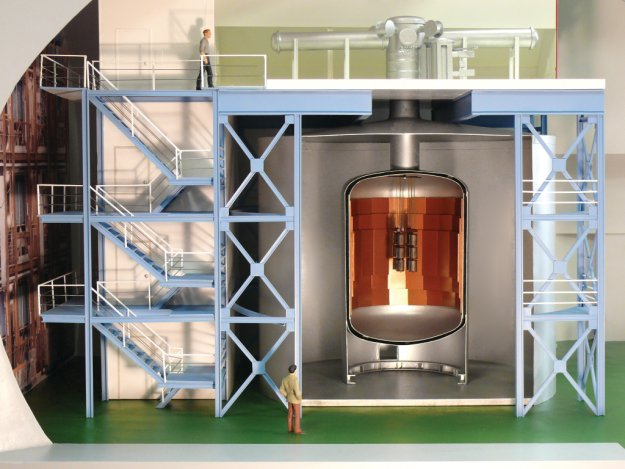
\includegraphics[width=\textwidth]{img/GERDAmodel}};
		\node(a) at (1.9,-1.5) [rectangle,draw,fill] {LAr};
		\node(b) at (4,1.6) [rectangle,draw,fill] {\ce{^76Ge} \textsc{detectors}};
		\draw[thick,red,->] (b.south) .. controls +(0,0) and +(1,0) .. (1.9,-0.4);
		\node(c) at (-1.5,1.6) [rectangle,draw,fill] {\textsc{water tank}};
		\draw[thick,red,->] (c.south) .. controls +(0,0) and +(-1,0) .. (0,-1);
		\node(d) at (0,3) [rectangle,draw,fill] {\textsc{copper shielding}};
		\draw[thick,red,->] (d.south) .. controls +(0,0) and +(-1,0) .. (1,0);
	\end{tikzpicture}
	\caption{Artists view (Ge array not to scale) of the Gerda experiment.}
	\label{artistview}
\end{figure}
\begin{figure}
	\centering
	\resizebox{\textwidth}{!}{
		\includegraphics[height=15cm]{img/strings}%
		\hspace{0.1cm}%
		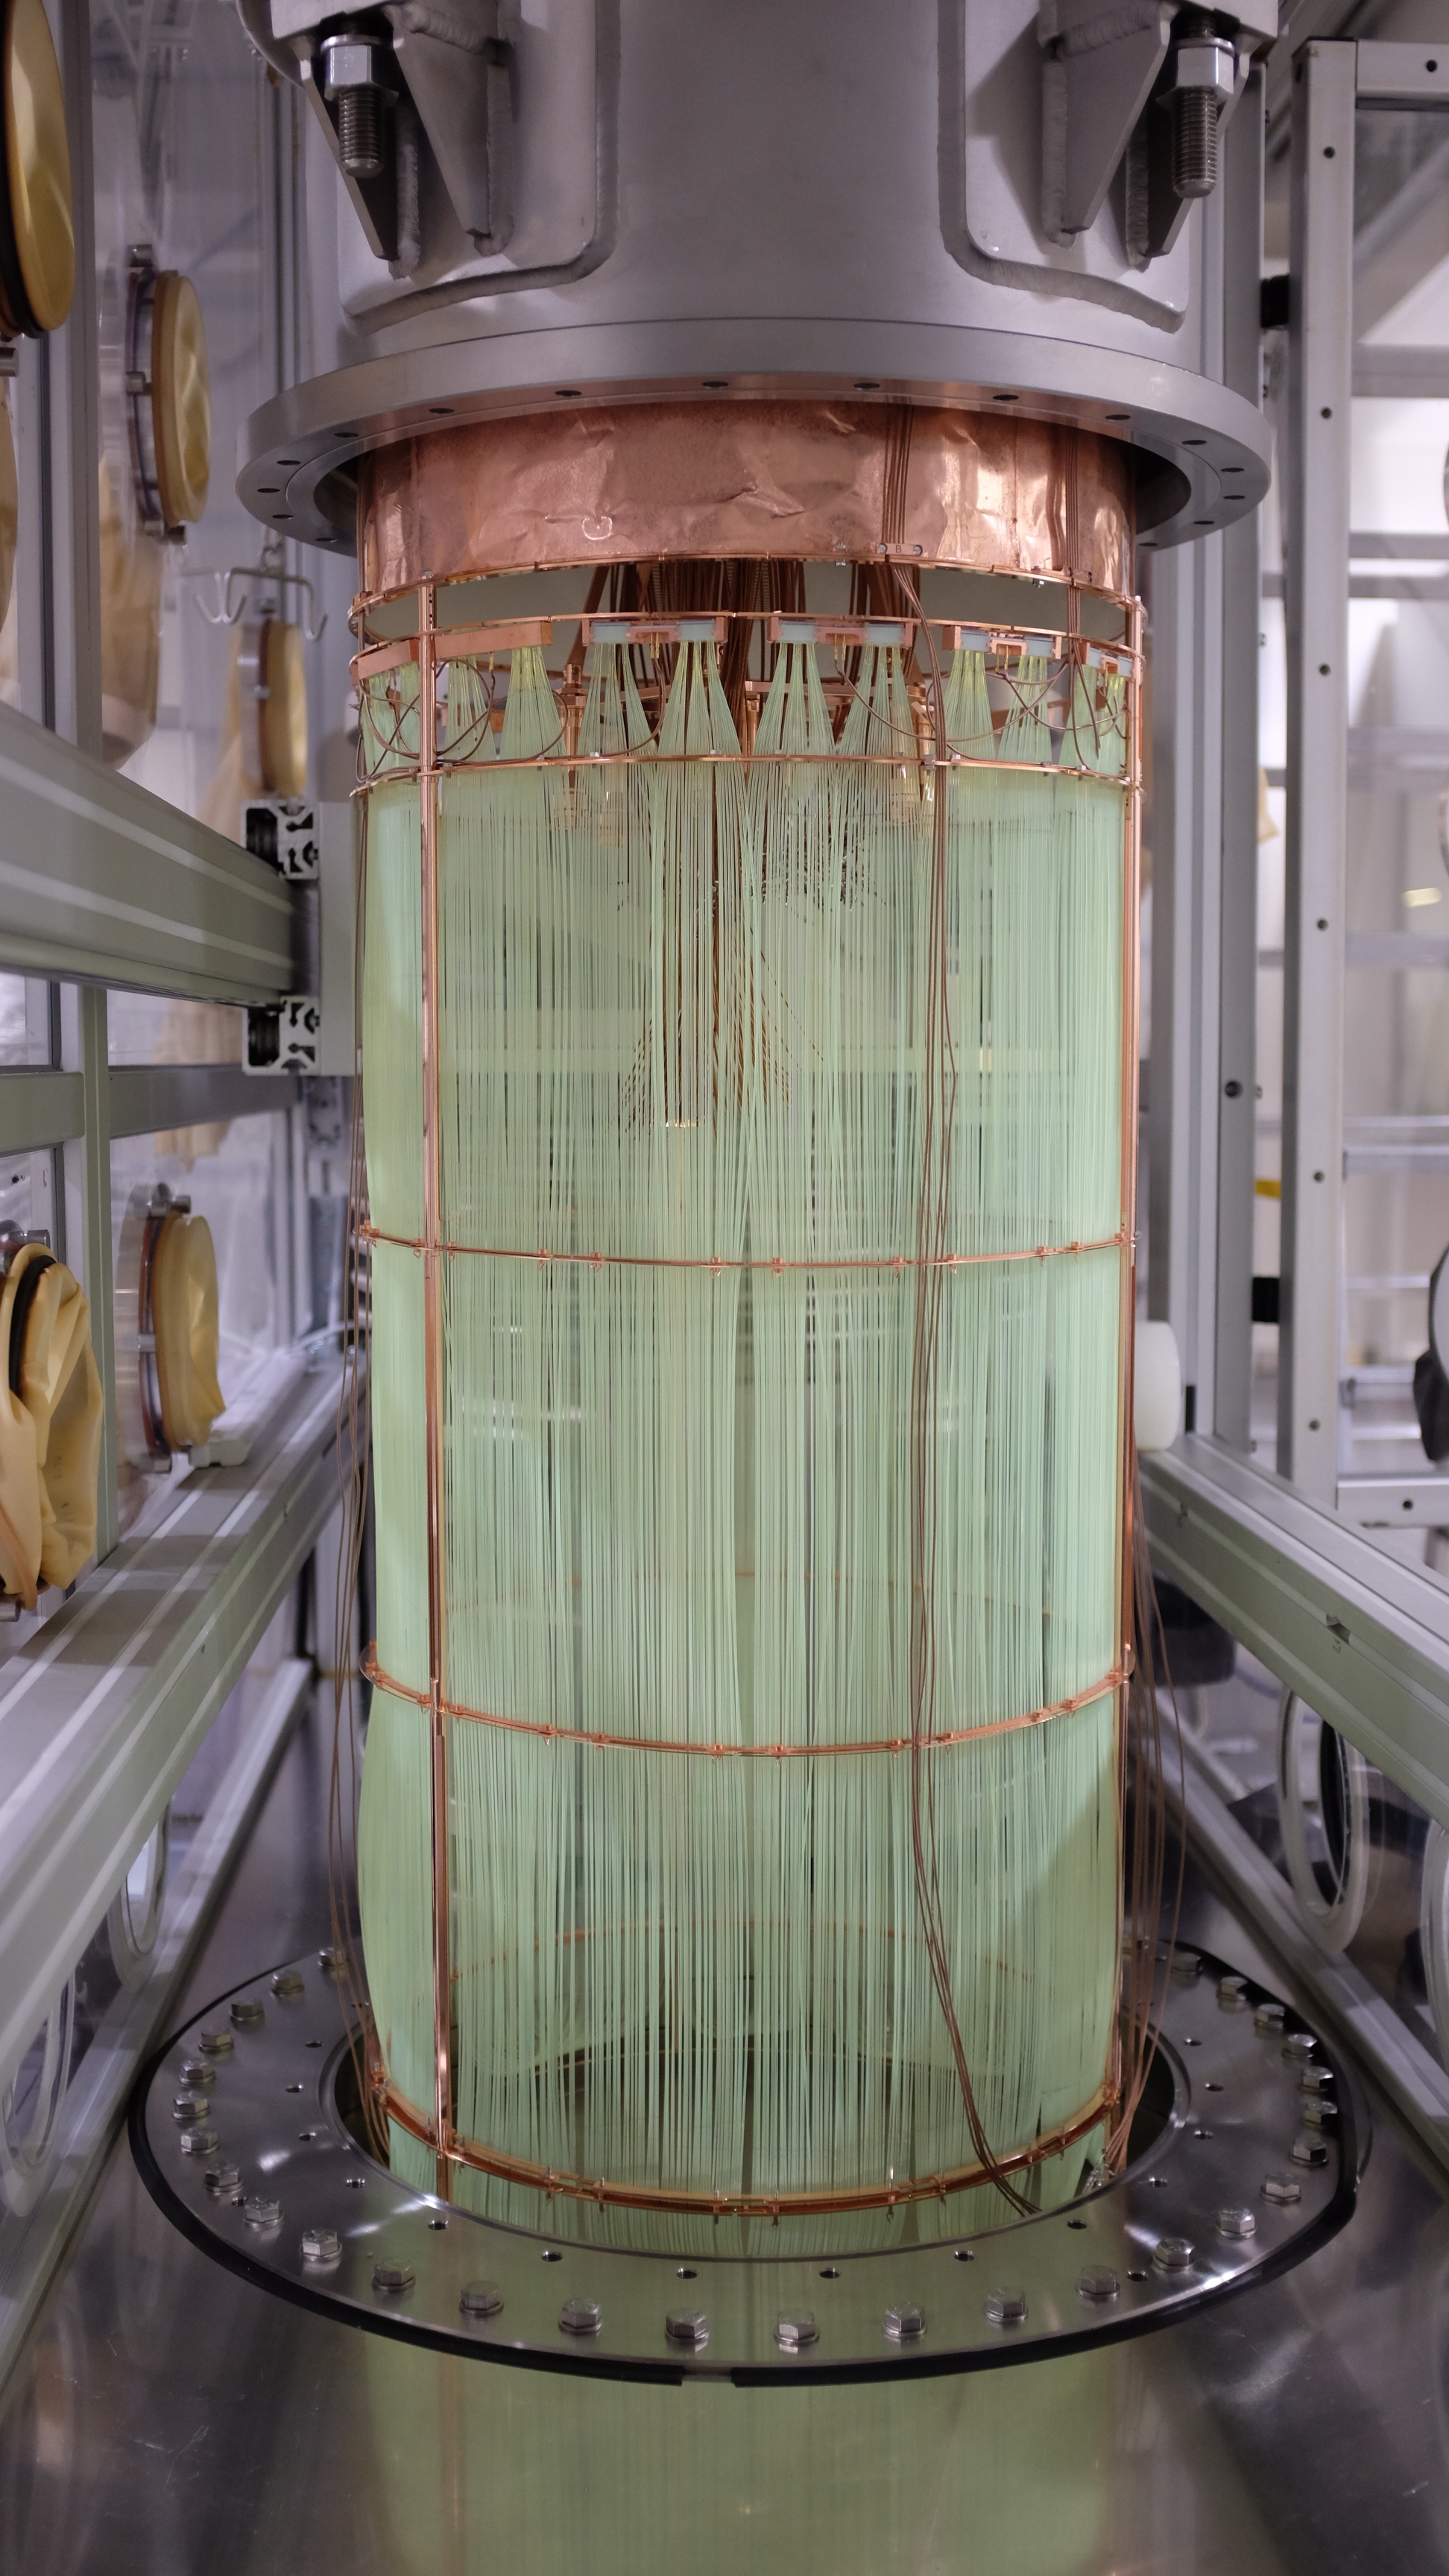
\includegraphics[height=15cm]{img/fibers}%
	}%
	\caption{On the left: some detector strings. On the right: the fiber shroud being submerged in LAr?}
\end{figure}
\begin{figure}
	\centering
	\makebox[\textwidth]{\includegraphics[width=\textwidth]{img/water_tank}}
	\caption{Inside the water tank after the installation of the muon veto system.}
\end{figure}

Fig.~\ref{artistview} shows a model of the realized design: the core of the experiment is an array of germanium diodes suspended in strings into a cryostat filled with LAr. The LAr serves both as cooling medium and shield. The cryostat is a steel vessel with a copper lining used primarily to reduce the gamma radiation from the steel vessel. The cryostat is placed in a large water tank, that fulfills the functions of shielding the inner volumes from radiation sources within the hall, such as neutrons, as well as providing a sensitive medium for a muon veto system. The detectors are lowered into the LAr volume using a lock system located in a clean room on top of the water tank. A further muon veto system is placed on top of the clean room in order to shield the neck region of the cryostat. A detailed description of the experimental setup for phase \textsc{i} is provided in \cite{gerdadescription}.

Phase \textsc{ii} came with some upgrades to improve the background rejection performance. The volume directly surrounding the detector array was instrumented with photo multipliers to detect the scintillation light emitted if energy is deposited inside LAr. This allows to identify background events resulting from Compton scattered photons with partial energy deposit in the detectors and partial energy deposit inside the LAr. Additionally, a curtain made from light guide fibers with tetraphenyl butadiene (TPB) deposited on their surface will surround the detector array. Photons reaching the light guides are wavelength shifted and guided to the end of the fibers, where they can be detected by silicon photomultipliers (SiPMs) optically coupled to the fibers. In principle the new components should improve the identification of background events. In Phase \textsc{i} the individual detector strings were surrounded by a copper shroud, minimizing the LAr volume from which \ce{^{42}K} ions can be collected on the detector surfaces. Additionally the shrouds were set to ground potential to minimize drift towards the detectors. In order to take maximum advantage of the light instrumentation of the LAr, in Phase \textsc{ii} the copper shroud has been be exchanged by a transparent TPB-coated shroud that allows to minimize the volume from which \ce{^{42}K} ions are collected, while allowing to detected scintillation light also from the volume inside the mini shroud. Last but not least, 30 new BEGe detectors were deployed into the LAr.

\marginnote{\textsc{The germanium detectors}} For Phase \textsc{i} all eight detectors from the former \textsc{HdM} \cite{hdm}and \textsc{Igex} \cite{igex} experiments were refurbished and redeployed, In addition, six detectors made of \ce{^{na}Ge} are available from the GENIUS-TF experiment \cite{genius1, genius2}. For Phase \textsc{ii} new material amounting to 50 kg \ce{^{enr}GeO2} was purchased in order to produce new diodes.

%! TEX root = ../main.tex
\chapter{The {\gerda} dataset and Monte Carlo simulations}
% {{{ THE GERDA DATA STRUCTURE
\marginnote{the\\{\gerda}\\data\\structure} In general the binary raw data format is custom defined by the different data acquisition systems. In order to optimize the analysis streaming and to provide a unique input interface for the analysis, all raw data are converted to a common standardized format. MGDO \cite{MGDO} (\textsc{Majorana} {\gerda} Data Objects) is a software library jointly developed by {\gerda} and \textsc{Majorana} \cite{majoranadem}. The core function of this software is to provide a collection of \texttt{C++} objects to encapsulate HPGe detector array event data and related analytical quantities. It also includes implementations of a number of general-purpose signal processing algorithms to support advanced detector signal analysis. The custom data objects available in the MGDO package are used as reference format to store events, waveforms, and other DAQ data (time stamps, flags). The MGDO data objects are stored as ROOT \cite{ROOT} files. The set of ROOT files produced by the conversion of raw data is named \textsc{Tier1}, and is officially distributed for the analysis.

Since the information contained in the \textsc{Tier1} set and in the raw data is expected to be equal, the conversion procedure is the optimal place where blinding can be applied. Events with an energy within $\pm$25 keV around $Q_{\beta\beta}$ are not exported to \textsc{Tier1} but they remain saved in the backup of the raw data.

The software framework \textsc{Gelatio} \cite{GELATIO} contains nearly independent and customizable modules that are applied to the input \textsc{Tier1} waveforms. The results (pulse amplitude, rise time, average baseline, energy, etc.) are stored as a new ROOT file (\textsc{Tier2}). A description of the analysis modules is presented in Ref.~\cite{dataproc}. Higher level \textsc{Tier}\emph{i} files that contain additional parameters evaluated from more advanced analysis (e.g.~calibrated energy spectra) can be created. In principle only the \textsc{Tier1} is official and every analysis should produce his own \textsc{Tier2} files depending on the actual needs. However there exists a `reference' \textsc{Tier2} produced with a standard set of \textsc{Gelatio} modules with a reasonable choice of parameters (e.g.~the width of the gaussian filter responsible for the reconstruction of the energy of an event) that can be used in most situations. The same reference datasets are provided for every \textsc{Tier}\emph{i} level.

Once the relevant quantities have been extracted from raw waveforms they have to be calibrated (e.g.~energy) and quality cuts (e.g.~for unphysical events) have to be applied. The results are again stored as a ROOT file (\textsc{Tier3}). The extraction of parameters related to the entire event (e.g.~the number of channels with a physical signal) is also performed at this level. Finally, high-level quality cuts are applied in \textsc{Tier4}, such as pulse shape discrimination, muon-veto and LAr-veto.

% }}}
% {{{ QUALITY CUTS
\marginnote{quality\\cuts} There is a set of classes of events that originates from failures in the acquisition process, limitations of the hardware components (e.g.~the FADC) or failures in the reconstruction process (\textsc{Gelatio}) and has to be excluded from the analysis. Also, there are events not related to an energy deposition, and thus consisting of a flat signal (an energy deposition in one detector triggers the sampling of the pulses from each of the 40 detectors, so it is very common to find pure-baseline signals in data), waveforms which amplitude exceeds the FADC's energy threshold (overshoot events), pile-up events, and all other unphysical events.

The main purpose for acquiring pulses from all the detectors when an energy deposition occurs anywhere is to provide the ability to discriminate multi-detector events. Such events cannot be associated to the double-beta decay electrons, which are absorbed within the detector's volume, and thus they can be discarded as background events. Events that leave a trace also in the water tank and/or in the upper scintillating panels and thus flagged by the muon-veto system are also discarded.

% }}}
% {{{ THE ENERGY SPECTRA
\marginnote{the\\energy\\spectra} With the cuts described above, the summed energy spectra from BEGe, enriched coaxial and natural coaxial detectors are presented in Fig.~\ref{fig:data}. The considered data set was taken between December 2015 and March 2017. Some prominent features can be identified. The low energy part up to 565 keV is dominated by $\beta^-$ decay of cosmogenic \ce{^{39}Ar} in all spectra. Slight differences in the spectral shape between the coaxial and BEGe type detectors result from differences in detector geometry and of the n$^+$ dead layer thickness. Between 600 and 1500 keV the spectra of the enriched detectors exhibit an enhanced continuous spectrum due to $2\nbb$ decay (see also Fig.~\ref{fig:energyspectra}). In all spectra, $\gamma$ lines from the decays of \ce{^{40}K} and \ce{^{42}K} can be identified, the spectra of the enriched coaxial detectors contain also lines from \ce{^{208}Tl} and \ce{^{214}Bi}. The peak-like structure around 3.5 MeV can be attributed to the $\alpha$-decays near the detector p$^+$ surface.

% }}}
\section*{Monte Carlo simulations}
Background components that were identified in the energy spectra or that were known to be present in the vicinity of the detectors were simulated using the \textsc{MaGe} \cite{MaGe} code based on \textsc{Geant4} \cite{geant4} and jointly developed by the {\gerda} and \textsc{Majorana} \cite{majoranadem} collaborations. The detectors and the arrangement of the germanium detector array with seven detector strings were implemented into the \textsc{MaGe} code as well as the other {\gerda} components (see Fig.~\ref{fig:volumes}). During the simulation \textsc{Geant4} generates complete information about the trajectory and interactions of particles as they propagate through the detectors. Although all of this information is available to the user, it is typically processed, parsed and saved to an output file for further analysis after the simulation run is complete. Simulations of contaminations of the following hardware components were performed: on the p$^+$ and n$^+$ surfaces of the detectors, homogeneously distributed in the LAr, in the detector assembly representing contaminations in the detector holders and their components, the mini shroud surrounding the detectors, the fiber shroud, the high-voltage cables and the signal cables. The volumes representing the germanium array, the holder mounting and the cables are simulated as depicted in Fig.~\ref{fig:volumes}. The mini shroud volume is implemented as a set of cylinders surrounding each detector string, while the fiber shroud consists of the lateral surface of a cylinder.
\begin{figure}
	\centering
	\resizebox{\textwidth}{!}{%
		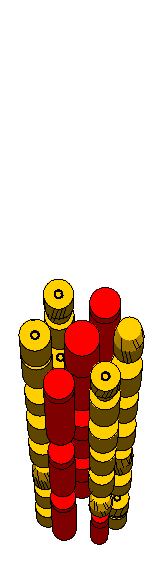
\includegraphics[]{img/gedet.pdf}%
		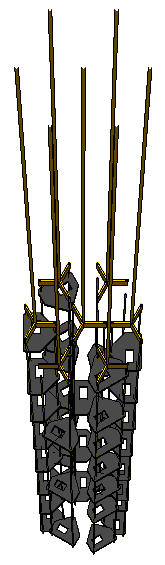
\includegraphics{img/holders.pdf}%
		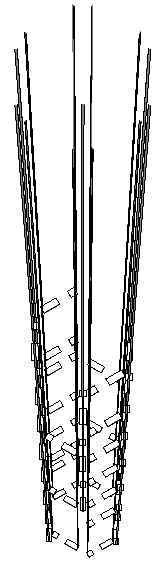
\includegraphics{img/cables.pdf}%
		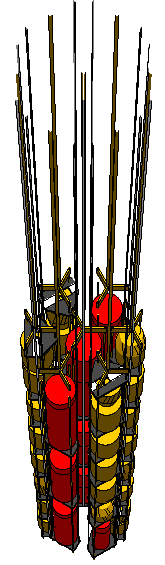
\includegraphics{img/all.pdf}%
	}%
	\caption{Implementation of the simulated volumes in \textsc{MaGe}. From left to right: the germanium detectors, the holder mounting, the cables and the three volumes put together.}\label{fig:volumes}
\end{figure}

% {{{ BACKGROUND INDEX
\marginnote{background\\index} The Background Index (BI), used to estimate the background activity in the \textsc{RoI}, is defined as the number of counts over detector's mass, live time and energy range inside a energy window defined as follows. The window covers the energy range between 1930 keV and 2190 keV excluding the blinded window around $Q_{\beta\beta}$. Also the two lines from \ce{^{208}Tl} and \ce{^{214}Bi} occurring respectively at 2104 keV and 2119 keV are neglected in this computation. This is done removing the energy range within $\pm$5 keV around the peaks. The width of the window is then 190 keV.

% }}}
% {{{ muons, neutrons, water tank
The expected background indices due to the neutron and muon fluxes at the LNGS underground laboratory have been estimated to be of the order < $10^{−5}$ cts/(keV$\cdot$kg$\cdot$yr) \cite{neutronsBI} and < $10^{−4}$ cts/(keV$\cdot$kg$\cdot$yr) \cite{muonsBI} respectively, and then are not considered. It has been also shown in earlier works that the contributions of the cryostat and water tank components are of the order < $10^{−4}$ cts/(keV$\cdot$kg$\cdot$yr) \cite{criowaterBI}, and then they have not been considered in this analysis.

% }}}
\begin{figure}
	\centerline{%
		\includestandalone[width=1.11\textwidth]{img/sim}\hspace{0.8cm}%
	}
	\caption{Simulated spectra. Top left: \ce{^{40}K}; top right \ce{^{42}K}; bottom left: $\alpha$-model; bottom right: {\color{red}Da completare}}
	\label{fig:simspectra}
\end{figure}
% {{{ 2nbb
\marginnote{$2\nbb$} The spectrum of the two electrons emitted in the $2\nbb$ decay of \ce{^{76}Ge} is sampled according to the distribution of \cite{tables2nbb} that is implemented in the code \textsc{decay0} \cite{decay0}. The $2\nbb$ decay distributions of \cite{tables2nbb} are in principle more precise than those based on the Primakoff-Rosen approximation, and they have been cross-checked against the high-statistics data of the \textsc{Nemo} experiment for several nuclei {\color{red}[ref?]}. Electrons are propagated in the {\gerda} simulated setup by \textsc{MaGe} and the total energy released in the active mass of the enriched detectors is registered.

% }}}
% {{{ 42Ar
\marginnote{\textnormal{\ce{^{42}Ar}}} While the distribution of \ce{^{42}Ar} is homogeneous inside LAr, the short lived ionized decay product \ce{^{42}K} ($T_{1/2} = 12.3$ h) can have a significantly different distribution due to drifts of the \ce{^{42}K} ions inside the electric fields that are present near the detectors. Separate spectra for two \ce{^{42}K} distributions have thus been simulated: homogeneous in LAr in a volume of centered around the full detector array, on the n$^+$ and on the p$^+$ detector surface of the detectors. As the spectral shape is not expected to vary strongly between the detectors, the isotope on the n$^+$ and p$^+$ surface was simulated only for a single detector. The simulated spectral shapes are shown in Fig.~\ref{fig:simspectra}.

% }}}
% {{{ 238U
\marginnote{\textnormal{\ce{^{238}U}}-chain} \ce{^{214}Bi} and \ce{^{214}Pb} are the only one in the \ce{^{226}Ra} $\rightarrow$ \ce{^{210}Pb} sub-chain decaying by $\beta$ decay accompanied by emission of high energy $\gamma$ particles and they are assumed to be in equilibrium. \ce{^{214}Bi} and \ce{^{214}Pb} were simulated in the holder mounting, in the cables, in the fiber shroud and in the mini shrouds. For the \ce{^{238}U} $\rightarrow$ \ce{^{226}Ra} the \ce{^{234\text{m}}Pa} was simulated, as the $Q_\beta$ of \ce{^{234}Th} is below the considered fitting range. {\color{red}giustificazione da ampliare}

% }}}
% {{{ 232Th
\marginnote{\textnormal{\ce{^{232}Th}}-chain} The characteristic $\gamma$ line at 2615 keV, a hint of the presence of isotopes from the \ce{^{232}Th} chain, can be clearly identified in the energy spectra shown in Fig.~\ref{fig:data}. Possible locations for contaminations are the detector assembly, the cables, the mini shrouds and the fiber shroud. As \ce{^{228}Ac} and \ce{^{228}Th} do not necessarily have to be in equilibrium, the two parts of the decay chain were simulated separately. From the sub-decay chain following the \ce{^{228}Th} decay only the contributions from the \ce{^{212}Bi} and \ce{^{208}Tl} decays were simulated, as theses are the only ones emitting high energetic $\gamma$ rays and electrons that can reach the detectors. {\color{red}giustificazione da ampliare}

% }}}
% {{{ 60Co
{\color{red}Manca 60Co}%\marginnote{\textnormal{\ce{^{60}Co}}}

% }}}
% {{{ 207Bi
{\color{red}Manca 207Bi}%\marginnote{\textnormal{\ce{^{207}Bi}}}

% }}}
% {{{ ALPHA MODEL
\marginnote{$\alpha$-model} From energies above 3.5 MeV the spectrum is dominated by $\alpha$-decay events, thus the background model in this region has been developed independently and then the resulting energy distribution has been added as a single contribution among the other background contributions.

A strong contribution from \ce{^{210}Po} can be observed in Fig.~\ref{fig:data}. This is indication for a surface contamination of the detectors. However, there are also hints for other peak like structures at 4.7, 5.4 and 5.9 MeV that can be attributed to the decays of \ce{^{226}Ra}, \ce{^{222}Rn} and \ce{^{218}Po} on p$^+$ detectors surfaces, respectively.

Due to the short range of $\alpha$-particles in germanium and LAr of the order of tens of $\mu$m, only decays occurring on or in the close vicinity (few $\mu$m) of the p$^+$ surface (assumed dead layer thickness roughly 300 nm) can contribute to the measured energy spectrum as the n$^+$ dead layer thickness is roughly 1 mm. The energy deposited in the active volume of the detector by surface or close to surface $\alpha$ particles is very sensitive to the thickness of the dead layer and on the distance of the decaying nucleus from the detector surface.

All $\alpha$-decays in the \ce{^{226}Ra} to \ce{^{210}Pb} sub-decay chain and the \ce{^{210}Po} decay have been simulated on the p$^+$ detector surface separately. Additionally, the decays in the chain following the \ce{^{226}Ra} decay were simulated assuming a homogeneous distribution in a volume extending up to 1 mm from the p$^+$ surface in LAr. The individual decays on the p$^+$ surface result in a peak-like structure with its maximum at slightly lower energies than the corresponding $\alpha$-decay energy with a quasi-exponential tail towards lower energy. The decays occurring in LAr close to the p$^+$ surface result in a quasi-flat spectrum without any peak-like structure extending to lower energies.

The \ce{^{210}Po} peak structure around 5.3 MeV with high statistics was used to determine the effective dead layer model. Spectra from \ce{^{210}Po} $\alpha$-decay simulations on the p$^+$ surface with different dead layer thicknesses were used to fit the spectrum in the energy region dominated by the \ce{^{210}Po} peak, i.e.~between 4850 and 5250 keV. The weight of each spectrum was left as a free parameter. A combination of the spectra for 300, 400, 500 and 600 nm dead layer thicknesses describes the observed peak structure well and results in a good fit, whereas a spectrum with a single dead layer thickness does not give a sufficiently good fit. Consequently the derived dead layer model was used for the later fits of $\alpha$-induced spectra.

In order to describe the whole energy interval dominated by $\alpha$-induced events, the simulated spectra of $\alpha$-decays of \ce{^{210}Po} as well as from \ce{^{226}Ra} and its short lived daughter nuclei on the p$^+$ surface and in LAr were used to fit the energy spectrum between 3500 and 7500 keV. In fact, while the surface decays alone can successfully describe the observed peak structures, they could not describe the whole spectrum. A contribution from an approximately flat component, like the spectra from $\alpha$-decays in LAr, is needed in the model. The number of events in the considered energy range was left as a free parameter for each $\alpha$ component.

% }}}
\section*{Screening measurements}
There are some radioactive contaminations in the components of {\gerda}, though not evident in the energy spectra, which have been identified and systematically measured. The most relevant contributions come from the silicon of the holder mounting, the cables, the nylon mini shroud covering the detectors and the fiber shroud.
\begin{table}
	\caption{Screening measurements for some of the considered {\gerda} components. The upper limits correspond to 90\% C.L.}
	\centerline{%
	\begin{tabular}{lcccccc}
		\toprule
		\multirow{2}{*}{Location}	&	\multicolumn{6}{c}{Activities [mBq/kg]} \\
		\cmidrule{2-7}
			&	\ce{^{40}K}	&	\ce{^{228}Th}	&	\ce{^{226}Ra}	&	\ce{^{60}Co}	&	\ce{^{234\text{m}}Pa}	&	\ce{^{228}Ra}	\\
		\midrule
		\textsc{fiber shroud}&&&&&&\\
		Fiber BCF-91A	&	0.46 $\pm$ 0.09	&	0.058 $\pm$ 0.012	&	--		&	--		&	0.042 (\ce{^{238}U})	&	--	\\
		\cmidrule{1-7}
		\textsc{holders}&&&&&&\\
		Si, V 3361/IKZ	&	4.3 $\pm$ 0.9	&	< 0.15	&	< 0.21	&	< 0.16	&	< 9.7 (\ce{^{238}U})	&	< 0.39	\\
		\cmidrule{1-7}
		\textsc{cables}&&&&&&\\
		Haefele 10 mils	&	109 $\pm$ 22	&	< 5.47	&	7.66 $\pm$ 2.2	&	--	&	< 365	&	< 8.4	\\
		Haefele 2 mils	&	222 $\pm$ 111	&	< 24.07	&	50 $\pm$ 11		&	--	&	< 2222	&	< 20.37	\\
		Tecnomec 3 mils	&	11 $\pm$ 3	&	< 0.46	&	< 0.38	&	--	&	< 44	&	< 0.56	\\
		\bottomrule
	\end{tabular}
	\label{tab:screening}
	}
\end{table}

{\color{red}spiegare come le misure sono state combinate, ho ancora dei dubbi su questo}\\
{\color{red}immagini catene di decadimento}
\begin{landscape}
\begin{figure}
	\centering
	\includestandalone{img/data}
	\caption{The summed energy spectrum (counts in logarithmic scale), showed separately for BEGe, enriched coaxial and natural coaxial detectors, produced using data from {\gerda} phase \textsc{ii}. The isotopes responsible for the relevant lines are reported on the plots together with the exposure. All the counts with energy greater than 3 MeV can be associated to $\alpha$ events on the p$^+$ electrode. The blinding window $\left[Q_{\beta\beta}-25\;\text{keV},Q_{\beta\beta}+25\;\text{keV}\right]$ is also shown in green. A 4 keV binning is adopted.}
	\label{fig:data}
\end{figure}
\end{landscape}

%%! TEX root = ../main.tex
\chapter{Statistical analysis}
A global model that describes the background spectrum was obtained by fitting the simulated spectra of different contributions to the measured energy spectrum using a Bayesian fit. A detailed description of the statistical method is given in the following.
\section*{A Bayesian approach}
The gist of Bayesian statistics is not difficult to grasp. At its base is the intuitive idea that probability quantifies the `degree of belief' in an event. The probability of an event changes if other events are assumed to be `true', provided these other events are `stochastically dependent' on that event. This is the essence of Bayes' theorem. As a consequence, Bayesian statistics allows the probability of a hypothesis to be continually updated on the basis of new observation (events) that depend on that hypothesis. 

% {{{ MODELING
\marginnote{modeling} The theory or model can be used to provide `direct probabilities'; i.e., relative frequencies of possible outcomes of the results were one to reproduce the experiment many times under identical conditions. The function $g(\vec{y}\mid\vec{\lambda},M)$ gives the relative frequency of getting results $\vec{y}$ assuming the model $M$ and parameters $\vec{\lambda}$. It should satisfy:
\[\int g(\vec{y}\mid\vec{\lambda},M)\text{d}\vec{y}=1 \quad\text{and}\quad g(\vec{y}\mid\vec{\lambda},M)>0\]
if continuous values are measured (in the discrete situation the integral gets replaced by a sum over all the possible outcomes). In the following, we will write formulae for the continuous case; the modification for the discrete case will be clear.

The prediction from the model cannot usually be directly compared to experimental results, the modeling of the experiment will usually add extra parameters and assumptions. We will use the symbol $\vec{\nu}$ to represent these additional nuisance parameters, which could also be limited by additional information not included explicitly in the model. In the following we will implicitly assume that all available information is used in the probability distributions. We would then have $f(\vec{x}\mid\vec{\lambda},\vec{\nu},M)$ for the frequency distribution of observable quantities $\vec{x}$.

In general, the judgement on the validity on a model and the extraction of values of the parameters within the model will be based on a comparison of the data $\vec{D}$ with $f(\vec{x}\mid\vec{\lambda},\vec{\nu},M)$.

% }}}
% {{{ THE LEARNING RULE
\marginnote{the\\learning\\rule} The probability of a model M will be quantified as $P(M)\in[0,1]$, while the probability density of the parameters are typically continuous functions. The parameters from the modeling of the experimental conditions are not correlated to the parameters of the physical model so that
\[P(\vec{\lambda},\vec{\nu}\mid M)=P(\vec{\lambda}\mid M)P(\vec{\nu})\;.\]
In the Bayesian approach the quantities $P(M)$ and $P(\vec{\lambda}\mid M)$ are treated as probabilities (probability densities), although they are not in any sense frequency distributions and are more accurately described as \emph{degrees-of-belief} \cite{bayesbook}. The \emph{degree-of-belief} contains out knowledge about nature and has to \emph{updated} by comparing data with the predictions of the model.

The procedure for learning from experiment is, according to the Bayes theorem:
\[P_{i+1}(\vec{\lambda},\vec{\nu},M\mid\vec{D})=\frac{f(\vec{x}=\vec{D}\mid\vec{\lambda},\vec{\nu},M)P_i(\vec{\lambda},\vec{\nu},M)}{\sum_M\int f(\vec{x}=\vec{D}\mid\vec{\lambda},\vec{\nu},M)P_i(\vec{\lambda},\vec{\nu},M)}\;,\]
where the index on $P$ represents the state-of-knowledge that gets updated from $i$ to $i+1$. The normalization factor derives from the normalization requirements on $P$ and we can also write it as $P(\vec{D})$, the probability to get the data $\vec{D}$.

For a given model $M$, $f$ is a function of the model parameters, the experimental parameters, and the possible outcomes $\vec{x}$. When $f$ is viewed as a function of $(\vec{\lambda},\vec{\nu})$ for fixed $\vec{x}=\vec{D}$, it is known as the likelihood. If $f$ is normalized, we can write
\[P(\vec{D}\mid\vec{\lambda},\vec{\nu},M)=f(\vec{x}=\vec{D}\mid\vec{\lambda},\vec{\nu},M)\;.\]

% }}}
% {{{ THE ROLE OF PRIORS
\marginnote{the role\\of priors} The presence of the prior distribution $P(\vec{\lambda},\vec{\nu},M)$ could generate suspects upon the statistical analysis `objectivity', in the sense that scientific conclusions may depend on `prejudices' about the value of a physical quantity. This is a logical necessity of the Bayesian approach, in which those who have done the experiment are the natural candidates to turn likelihoods in probabilistic statements.

At an intuitive level, it is absolutely reasonable to draw conclusions starting from some prior knowledge, rather than in a purely automatic way. For example, in the most extreme case, if the experimental information is scarce or doubtful it is absolutely right to believe more in personal prejudices than in empirical data. Moreover, if different observers have priors which are so different that they reach divergent conclusions, it just means that the data are still not sufficiently solid to allow a high degree of intersubjectivity and we are on a sticky ground. Thus, one is expected to use different prior distributions to test the robustness of his probability statements \cite{bayesbook}.

% }}}
% {{{ PARAMETER ESTIMATION
\marginnote{parameter\\estimation} Parameter estimation is performed while keeping the model fixed. It this case we write
\begin{equation}P(\vec{\lambda},\vec{\nu}\mid\vec{D},M)=\frac{P(\vec{x}=\vec{D}\mid\vec{\lambda},\vec{\nu},M)P_0(\vec{\lambda},\vec{\nu}\mid M)}{\int P(\vec{x}=\vec{D}\mid\vec{\lambda},\vec{\nu},M)P_0(\vec{\lambda},\vec{\nu}\mid M)}\;,\label{eq:posterior}\end{equation}
The output of the evaluation is a normalized probability density for the parameters, including all correlations, and hence it can be used to give best-fit values, probability intervals for the parameters, etc.

When working with the posterior probability density function (or \emph{pdf}) \ref{eq:posterior}, it is often the case that one is interested not in the full \emph{pdf}, but in the probability distribution for only one, or a few, parameters. These distributions are determined via marginalization. For example, the probability distribution for parameter $\lambda_i$ is:
\[P(\lambda_i\mid\vec{D},M)=\int P(\vec{\lambda},\vec{\nu}\mid\vec{D},M)\text{d}\vec{\lambda}_{i\neq j}\text{d}\vec{\nu}\;.\]
Note that the parameter values which maximize the full posterior \emph{pdf} usually do not coincide with the values which maximize the marginalized distributions.

We will mainly interested in estimating the mode of $\lambda_i$, i.e.~the value of $\lambda_i$ which maximizes the marginalized posterior \emph{pdf}
\[\text{argmax}\left[ P(\lambda_i\mid\vec{D},M) \right]\]
and confidence intervals such that a certain fraction $\alpha$ of the total area is contained in it:
\[\alpha=\int^{\lambda_\text{upper}}_{\lambda_\text{lower}}P(\lambda_i\mid\vec{D},M)\text{d}\lambda_i\;,\]
where the desired interval is $[\lambda_\text{lower},\lambda_\text{upper}]$.

% }}}
% {{{ MODEL VALIDITY
\marginnote{model\\validity} Model testing in a strictly Bayesian approach is problematic since there is often no way to define all possible models, and the results depend critically on the choice of priors. However, having a number representing how well the model fits the available data is important. Here we consider a p-value that gives a goodness-of-fit criterion based on the likelihood of the data in the model under consideration using the parameters defined at the mode of the posterior. We define the following function:
\[\hat{f}(\vec{x})=P(\vec{x}\mid\hat{\vec{\lambda}},\hat{\vec{\nu}},M)\;,\]
where $(\hat{\vec{\lambda}},\hat{\vec{\nu}})$ is the set of parameters at the mode of the full \emph{pdf}. We then define the p-value as
\[p=\frac{\int_{\hat{f}(\vec{x})<\hat{f}(\vec{D})}\hat{f}(\vec{x})\text{d}\vec{x}}{\int \hat{f}(\vec{x})\text{d}\vec{x}}\;.\]
$p$ is the tail area probability to have found a result with $\hat{f}(\vec{x})<\hat{f}(\vec{D})$, assuming that the model $M$ is valid and all experimental effects are perfectly known. It is the probability that the likelihood could have been lower than the observed in the data, so it the model does not give a good representation of the data, then $p$ will be a small number. If the modeling is correct, $p$ will have a flat probability distribution in $[0,1]$, but it should be clear that incorrect formulations of the data fluctuations will bias the p-value distribution to lower (if the data fluctuations are underestimated) or higher (if the data fluctuations are overestimated) values. Also, if the existing data are used to modify the parameter values, the extracted p-value will be biased to higher values.

One should also keep in mind that p-values cannot be turned into probabilistic statements about the model being correct without priors, and should therefore be handled with care. General guidelines suggest that one should check if the p-value distribution is reasonably flat, keeping in mind that sharply falling distributions starting at $p=0$ are usually originated by a bad model. Moreover, small p-values are worrisome, they indicate that a poor model might has been picked. For further discussions on the topic see, for example, \cite{p-value}.

% }}}
% {{{ COMPUTATIONAL ASPECTS
\marginnote{computational\\aspects} There are several ways to calculate the posterior in \ref{eq:posterior} and the marginalized \emph{pdf}s, and even with few parameters $(\vec{\lambda},\vec{\nu})$ the computation can easily become highly time consuming. However, the application of Markov Chain Monte Carlo (MCMC) methods in this field has revolutionized Bayesian computation. The BAT package \cite{BAT} implements several tools to perform a Bayesia data analysis.

Markov chains are sequences of random numbers (or, in general, vectors of numbers), $X_t$, which follow a well-defined limiting distribution, $\pi(x)$. The fundamental property of a Markov chain is that the probability distribution for the next element in the sequence, $X_{t+1}$, depends only on the current state, and not on any previous history. A Markov chain is completely defined by the one-step probability transition matrix, $P(X_{t+1}\mid X_t)$. Under certain conditions (recurrence, irreducibility, aperiodicity), it can be proven that the chain is ergodic; i.e., that the limiting probability to be in a given state does not depend on the starting point of the chain. An MCMC is an algorithm producing an ergodic Markov chain which stationary distribution is the distribution of interest. In our case, the BAT package produces a Markov chain where the stationary distribution is the desired posterior \emph{pdf}.

A very popular algorithm that achieves this is the Metropolis-Hastings algorithm \cite{Metropolis,Hastings}. The algorithm works as follows:
\begin{enumerate}
	\item Given the system in a starting state $X_t=\vec{x}$, a new proposed state $\vec{y}$ is generated according to a symmetric proposal function $g(\vec{y},\vec{x})$ (in our application a state is a set of parameter values);
	\item The Hastings test ratio
		\[r=\text{min}\left[1,\frac{\pi(\vec{y})}{\pi(\vec{x})}\right]\]
		is calculated, and then the generated state $\vec{y}$ is accepted or rejected with probability $r$, i.e.:
		\begin{enumerate}
			\item Generate a random number $u$ from a uniform distribution between $0$ and $1$, $\text{Unif}[0,1]$;
			\item If $u<r$ set $X_{t+1}=\vec{y}$, else take $X_{t+1}=\vec{x}$.
		\end{enumerate}
\end{enumerate}
It is possible to show that, given a reasonable proposal function $g$, this algorithm satisfies the conditions of an MCMC, and that the limiting distribution is $\pi(\vec{x})$. Thus this allows for the production of states distributed according to the desired distribution.

% }}}
% {{{ IMPLEMENTATION
\marginnote{implementation} The BAT software is \texttt{C++} based code interfaced to software packages such as ROOT \cite{ROOT}, \textsc{Minuit} \cite{MINUIT}, or the CUBA library \cite{CUBA}. Several Markov chains can optionally be run in parallel thanks to the OpenMP \cite{openmp} support. For further details about the statistical theory and implementation aspects, as well as applications to real problems, underlying the BAT package see \cite{BAT}, for a detailed description of the class structure and the methods the official documentation is available at \texttt{http://www.mppmu.mpg.de/bat/}.

% }}}
\section*{Background decomposition}
The analysis of the energy distributions was carried out by fitting binned energy distributions. The likelihood $P(\vec{D}\mid\vec{\lambda})$ is written as the product of the probability of the data given the model and parameters in each bin:
\[P(\vec{D}\mid\vec{\lambda})=\prod_i^{N}P(n_i\mid\mu_i)=\prod_i^N\frac{e^{-\mu_i}\mu_i^{n_i}}{n_i!}\;,\]
where $N$ is the number of bins, $n_i$ is the observed number of events and $\mu_i$ is the expected number of events (frequency) in bin $i$. $\mu_i$ can be written as the sum of the background contributions in bin $i$:
\[\mu^i=\sum_jb_j^i=\sum_j c_jh_j^i\;,\]
where the index $j$ runs over all the background contributions and $b_j^i$ is the expected number of events for the background source $j$ in bin $i$. The latter can be further decomposed in the product of the frequency $h_j^i$ in bin $i$ and a factor $c_j$, which does not depend on the bin and contains the $\lambda_j$ parameter of physical interest that will be estimated with the fitting procedure.

We want to keep the summed energy spectra from BEGes and coaxial separate, as the contamination of radioactive sources on the electrodes can be different. All the other parameters (e.g. the double-beta decay half-life or the \ce{^{60}Co} activity in the detector assembly) are the same for the two spectra. The natural coaxial detectors were omitted from the analysis because the contribution to the double-beta decay spectrum is too small to be relevant. Then the likelihood can be expressed as
\[P(\vec{D}\mid\vec{\lambda})=P_\text{BEGe}(\vec{D}\mid\vec{\lambda})P_\text{Coax}(\vec{D}\mid\vec{\lambda})=\prod_i^N\left[\frac{e^{-\mu_i}\mu_i^{n_i}}{n_i!}\right]_\text{BEGe}\prod_j^N\left[\frac{e^{-\mu_j}\mu_j^{n_j}}{n_j!}\right]_\text{Coax}\]

% {{{ 2nbb
\marginnote{$2\nbb$} For the two-neutrino mode of double-beta decay we want to estimate the half-life $T_{1/2}$. In this case the contribution $b_{2\nu}^i$ can be written as
\[b_{2\nu}^i=\frac{N_A\log2}{A_{76}T_{1/2}}\sum_{k=1}^\text{det}m_kt_kf^{76}_k\left[\epsilon^i_kf^i\right]_{2\nu}\;,\]
where $k$ labels the detectors, $N_A$ is the Avogadro number, $A_{76}$ is the molar weight of \ce{^{76}Ge}, $f^{76}$ is the enrichment fraction, and $t$ is the detector's live time. The detection efficiency $\epsilon_{2\nu}^{ik}$ has to be intended as a generalized efficiency which comprises the effect of the presence of the dead layer and the intrinsic efficiency of the detector $k$. $f_{2\nu}^i$ is the theoretical absolute frequency (i.e.~the entire distribution is normalized to one) for double-beta decay in bin $i$, it is the discrete version of \ref{eq:spectstd}. We adopted the approximation $T_{1/2}\gg t$.

The expression holds also for the Lorentz-violating mode, with the associated half-life $T_{1/2}^\text{LV}$. Recalling the equation \ref{eq:totwidth} we can express $T_{1/2}^\text{LV}$ in relation to $T_{1/2}$ and $\aof$:
\[T_{1/2}^\text{LV}=I\cdot\frac{T_{1/2}}{\aof}\qquad I=\frac{10}{\aof}\frac{\int_0^{K_0}\frac{\text{d}\delta\Gamma}{\text{d}K}\text{d}K}{\int_0^{K_0}\frac{\text{d}\Gamma_0}{\text{d}K}\text{d}K}\;,\]
and then the $b_{2\nu\text{LV}}^i$ factor can be written as:
\[b_{2\nu\text{LV}}^i=\frac{\aof}{I}\frac{N_A\log2}{A_{76}T_{1/2}}\sum_{k=1}^\text{det}m_kt_kf^{76}_k\left[\epsilon^i_kf^i\right]_{2\nu\text{LV}}\;,\]

% }}}
% {{{ EXTERNAL SOURCES
\marginnote{external\\sources} For the other background sources the parameter of interest is the activity, defined as the number of events per unit of time and mass. Assuming a stable isotope contamination within the considered live times, we can express $b_j$ as
\[b_j^i=a_jM\sum_k^\text{det}t_k\epsilon_j^{ik}f_j^i\;,\label{eq:extsources}\]
where $a_j$ is the activity for the source $j$ and $M$ is the mass of the object in which the source is located. The detection efficiency $\epsilon_j^{ik}$ has to be intended as a generalized efficiency which comprises the effect of the presence of the dead layer, the intrinsic efficiency and the solid angle the detector $k$ subtends at the radioactive source.

It should be noted that the activities of some isotopes are correlated, for example if they come from the same decay chain. In this analysis we have two examples of this, \ce{^{212}Bi} decays in \ce{^{208}Tl} with 39.93\% branching ratio, while \ce{^{214}Pb} decays in \ce{^{214}Bi} with $\sim$100\% branching ratio.

% }}}
% {{{ SIMULATED SPECTRA
\marginnote{simulated\\spectra} The simulated spectra, for $2\nbb$ and background sources, come from \textsc{MaGe} in the form
\[b^{ik}_{\textsc{MaGe},j}=N_\text{gen}\epsilon^{ik}_jf_j^i\;,\]
where $N_\text{gen}$ is the number of primary vertices simulated and $i$, $j$, $k$ label the $i$-th bin, the source and the detector, respectively. The spectra for each detector have then to be combined properly in order to be fitted to the data. In the case of external sources, for example, the form in equation \ref{eq:extsources} has to be reproduced rescaling each spectra with $N_\text{gen}$, then multiplying by $t_k$ and $M$ and finally summing over all detectors. Then the overall factor $\lambda_i$ will be the parameter to estimate with the fitting procedure:
\[b_{\text{sim},j}^i=\lambda_jM\sum_k^\text{det}t_k\epsilon_j^{ik}f_j^i\;.\]


% }}}

\bibliographystyle{unsrt}
\bibliography{bib-thesis}
\end{document}
